\newcommand{\basedir}{fablab-document}
\documentclass{\basedir/fablab-document}

\usepackage{minitoc} % Inhaltsübersicht je Section
% \usepackage{fancybox} %ovale Boxen für Knöpfe - nicht mehr benötigt
\usepackage{amssymb} % Symbole für Knöpfe
% \usepackage{subfigure,caption}
\usepackage{eurosym}
\usepackage{tabularx} % Tabellen mit bestimmtem Breitenverhältnis der Spalten
\usepackage{wrapfig} % Textumlauf um Bilder
\usepackage{todonotes}
\usepackage{multirow}
\usepackage{framed}
\usepackage{xargs}
\usepackage{caption}

\renewenvironmentx{leftbar}[3][2=0.5pt, 3=5pt]{\def\FrameCommand{\vrule width #2 \hspace{#3}}\MakeFramed {\advance\hsize-\width \FrameRestore}{\tiny#1\\}} {\endMakeFramed}

\renewcommand{\texteuro}{\euro}

\linespread{1.2}

\date{Oktober 2015}
\author{}
\title{Einweisung Kreissäge}

\begin{document}
 % Hinweise an Package minitoc, doch bitte irgendwas zu generieren - wird für späteres \secttoc benötigt
\dosecttoc
\faketableofcontents
\mtcsettitle{secttoc}{Arbeitsschritte}
\mtcsettitlefont{secttoc}{\large \sffamily \bfseries}
\mtcsetfont{secttoc}{subsection}{\sffamily}
% \mtcset
% hier geht das eigentliche Dokument los

%\color{red}
%\hrule
%\begin{center}
%\large{Achtung! Einweisung ist noch in Arbeit!}
%\vspace{0.1cm}
%\end{center}
%\hrule
%\color{black}

\section{Technische Daten}
\begin{tabular}{r|l}
Hersteller & Festool \\
Produktname & Tauchsäge TS 55 REBQ \\
Leistung & $1200\,\mathrm{Watt}$ \\
Drezahlbereich & $2.000 - 5.800\,\mathrm{min}^{-1}$ \\
\multirow{2}{*}{Schnitttiefe} & max. $55\,\mathrm{mm}$ \\
             & max. $43\,\mathrm{mm}$ bei 45º\\
Sägeblattabmessung & $160\times 2,2\times 20\,\mathrm{mm}$\\
\end{tabular}

\section[Allgemeine Sicherheitshinweise]{Allgemeine Sicherheitshinweise}

Dieser Abschnitt nennt die wichtigsten Gefahren und Sicherheitsregeln.

\textbf{Gefahr durch das Sägeblatt: Sägen von Fingern, Beinen, der Arbeitsplatte, ...}
\begin{itemize}
\item Hände bei aktiver Säge immer vom Sägebereich und dem Sägeblatt fernhalten. Die Kreissäge immer mit beiden Händen halten. Wenn beide Hände die Kreissäge halten, kann das Sägeblatt diese nicht verletzen.

\item Nicht unter das Werkstück greifen. Die Schutzhaube kann unterhalb des Werkstückes nicht vor dem Sägeblatt schützen.

\item Die Schnitttiefe an die Dicke des Werkstücks anpassen. Es sollte weniger als eine volle Zahnhöhe unter dem Werkstück sichtbar sein. Es darf nicht tiefer als 1\,mm in den Festool-Arbeitstisch gesägt werden.

\item Das Werkstück muss fest und sicher verspannt sein.

\item Auf keinen Fall so sägen, dass das Stromkabel getroffen werden kann. Die Metallteile des Elektrowerkzeugs könnten sonst unter Spannung stehen und einen elektrischen Schlag verursachen.

\item Bei beschädigtem Stromkabel die Arbeit sofort beenden, Stecker ziehen und Anschlusskabel gegen ein intaktes auswechseln.
\end{itemize}

\textbf{Gefahr des Wegschleuderns von Werkstückteilen}
\begin{itemize}
\item Das Werkstück stabil und sicher fixieren, z.\,B. mit Schraubzwingen auf dem Festool Arbeitstisch. Dies ist wichtig,
um die Gefahr von Körperkontakt, Klemmen des Sägeblattes oder Verlust der Kontrolle zu minimieren.

\item Immer die Führungsschiene verwenden. Soweit möglich, diese mit den dafür vorgesehenen Schraubzwingen am Werkstück oder Arbeitstisch befestigen. Dies verbessert die Schnittgenauigkeit und verringert die Möglichkeit, dass das Sägeblatt klemmt.

\item Nur passende Sägeblätter und -Spannflansche von Festool verwenden (siehe Bedienungsanleitung).

\item Im Arbeitsbereich dürfen sich keine Unbeteiligten befinden. Die Benutzung innerhalb des FabLabs während normaler Öffnungszeiten ist nicht möglich.
\end{itemize}

\textbf{Rückschlagen der Säge}
\begin{leftbar}{Aus Festool TS 55 REBQ Handbuch, Abschnitt 2.2 (Anmerkungen in Abschnitt~\ref{quellen} beachten)}
Ein Rückschlag ist die plötzliche Reaktion
eines hakenden, klemmenden oder falsch
ausgerichteten Sägeblattes, die dazu führt,
dass eine unkontrollierte Säge abhebt und
sich aus dem Werkstück heraus in Richtung der Bedienperson bewegt.\\
Ein Rückschlag ist die Folge eines falschen
oder fehlerhaften Gebrauchs der Säge. Er kann
durch geeignete Vorsichtsmaßnahmen, wie
nachfolgend beschrieben, verhindert werden.
\begin{itemize}
\item Halten Sie die Säge mit beiden Händen
fest und bringen Sie Ihre Arme in eine
Stellung, in der Sie die Rückschlagkräfte
abfangen können. Halten Sie sich immer
seitlich des Sägeblattes, nie das Sägeblatt
in eine Linie mit Ihrem Körper bringen. 
\item Falls das Sägeblatt verklemmt oder Sie
die Arbeit unterbrechen, lassen Sie den
Ein-/Ausschalter los und halten Sie die
Säge im Werkstoff ruhig, bis das Sägeblatt
vollständig zum Stillstand gekommen ist.
Versuchen Sie nie, die Säge aus dem
Werkstück zu entfernen oder sie rückwärts zu ziehen, solange das Sägeblatt
sich bewegt, sonst kann ein Rückschlag
erfolgen.
\item Wenn Sie eine Säge, die im Werkstück
steckt, wieder starten wollen, zentrieren
Sie das Sägeblatt im Sägespalt und überprüfen Sie, ob die Sägezähne nicht im
Werkstück verhakt sind. 
\item Stützen Sie große Platten ab, um das Risiko eines Rückschlags durch ein klemmendes Sägeblatt zu vermindern.

\end{itemize}
\end{leftbar}

\textbf{Gesundheitsgefahr durch Holzstaub}
\begin{itemize}
	\item Immer Staubsauger anschließen. Nur den für Staubklasse M zugelassenen Festool Staubsauger verwenden.
	\item Bei Hartholzbearbeitung im FabLab ist darauf zu achten, dass kein Hartholzstaub entsteht. Falls doch, darf die Arbeit im FabLab nicht fortgesetzt werden. Abhilfe kann ein Umzug nach draußen schaffen.
\end{itemize}

\textbf{Wenn bei der Benutzung ein Schaden an der Maschine entsteht, ist dieser und der Hergang unverzüglich über Mail an fablab-aktive@fablab.fau.de zu mailen!}

\subsection{Schutzausrüstung}

\begin{itemize}
\item Gehörschutz (befindet sich bei der Fräse)
\item Schutzbrille bei Metallbearbeitung (neben der Fräse über der Werkbank)
\item Staubmaske bei stauberzeugenden Arbeiten (insbesondere Hartholz)
\item Schutzhandschuhe beim Bearbeiten rauer Materialien und beim Werkzeugwechsel tragen.
\item eng anliegende Kleidung ohne Fransen oder Abstehende Elemente wie Kordeln etc. (kann in rotierende Maschine eingezogen werden)
\item bei längeren Haaren: keine offenen Haare
\end{itemize}

\section{Bestimmungsgemäße Verwendung}
Tauchsägen sind bestimmungsgemäß zum Sägen von Holz, holzähnlichen Werkstoffen, gips- und zementgebundenen Faserstoffen sowie Kunststoffen vorgesehen. Hierfür ist auf die richtige Auswahl des Sägeblattes zu achten. Mit den von Festool angebotenen Spezialsägeblättern für Aluminium können die Maschinen auch zum Sägen von Aluminium verwendet werden. Es dürfen nur Sägeblätter gemäß der Bedienungsanleitung verwendet werden.
\begin{itemize}
\item Die Tauchsäge darf ausschließlich von eingewiesenen Personen verwendet werden.
\item Diese Einweisung bezieht sich auf die Verwendung als Tauchsäge mit Führungsschiene zum Zersägen von Plattenmaterial, Holzlatten und ähnlichem. Andere Einsätze, etwa die freihändige Benutzung, sind nicht gestattet.
\end{itemize}

\subsection{Aluminiumbearbeitung}
Bei der Bearbeitung von Aluminium sind aus Sicherheitsgründen folgende besonderen Maßnahmen einzuhalten:
\begin{itemize}
\item Maschine an ein geeignetes Absauggerät anschließen.
\item Maschine regelmäßig von Staubablagerungen im Motorgehäuse reinigen.
\item Nur Aluminium-Sägeblätter verwenden.
\item Sichtfenster / den Spanflugschutz schließen. Schutzbrille oder Schutzschild nutzen!
\end{itemize}


\section{Inbetriebnahme}
Maschine vor dem Anschließen und Lösen der Netzanschlussleitung stets ausschalten! Anschließen und Lösen der Netzanschlussleitung siehe Bild [2].
Schieben Sie die Einschaltsperre nach oben und drücken Sie den Ein-/Ausschalter (drücken = Ein / loslassen = AUS).
Die Betätigung der Einschaltsperre entriegelt die Eintauchvorrichtung. Das Sägeaggregat kann nach unten bewegt werden. Dabei taucht das Sägeblatt aus der Schutzhaube aus.

\section{Arbeiten mit der Säge}
\begin{leftbar}{Aus Festool TS 55 REBQ Handbuch, Abschnitt 8 (Anmerkungen in Abschnitt~\ref{quellen} beachten)}
Beachten Sie beim Arbeiten alle eingangs gemachten Sicherheitshinweise
sowie folgende Regeln:
\begin{itemize}
\item Führen Sie das Elektrowerkzeug nur im
eingeschalteten Zustand gegen das Werkstück.
\item Kontrollieren Sie vor jedem Einsatz die
Funktion der Einbauvorrichtung und verwenden Sie die Maschine nur, wenn diese
ordnungsgemäß funktioniert.
\item Befestigen Sie das Werkstück stets so,
dass es sich beim Bearbeiten nicht bewegen kann.
\item Halten Sie das Elektrowerkzeug beim Arbeiten immer mit beiden Händen an den
Handgriffen [1-4]. Dies vermindert die Verletzungsgefahr und ist die Voraussetzung
für exaktes Arbeiten.
\item Schieben Sie die Säge stets nach vorne [9-2], keinesfalls rückwärts zu sich heranziehen.
\item Vermeiden Sie durch eine angepasste Vorschubgeschwindigkeit eine Überhitzung
der Schneiden des Sägeblattes, und beim
Schneiden von Kunststoffen ein Schmelzen
des Kunststoffes.
\item Vergewissern Sie sich vor dem Arbeiten,
dass alle Drehknöpfe [4-1] fest angezogen
sind.
\item Arbeiten Sie nicht mit der Maschine, wenn
die Elektronik defekt ist, da dies zu überhöhten Drehzahlen führen kann. Eine fehlerhafte Elektronik erkennen Sie am fehlenden Sanftanlauf oder wenn keine Drehzahlregelung möglich ist.
\end{itemize}
\end{leftbar}

\section{Einstellungen}
\subsection{Funktionen der Maschine}
\begin{itemize}
\item Sanftanlauf: Der elektronisch geregelte Sanftanlauf sorgt für ruckfreien Anlauf des Elektrowerkzeugs.
\item Konstante Drehzahl: Die Motordrehzahl wird elektronisch konstant gehalten. Dadurch wird auch bei Belastung eine gleichbleibende Schnittgeschwindigkeit erreicht.
\item Drehzahlregelung: Die Drehzahl lässt sich mit dem Stellrad stufenlos einstellen. Siehe Tabelle \ref{fig:drehzahltabelle}.
\item Temperatursicherung: Bei zu hoher Motortemperatur werden Stromzufuhr und Drehzahl reduziert. Die Maschine läuft nur noch mit verringerter Leistung, um eine rasche Abkühlung durch die Motorlüftung zu ermöglichen. Wenn die Übertemperatur andauert, schaltet die Maschine nach ca. 40 sec komplett ab. Erst nach Abkühlung des Motors ist ein erneutes Einschalten möglich.
\item Strombegrenzung: Die Strombegrenzung verhindert bei extremer Überlastung eine zu hohe Stromaufnahme. Dies kann zu einer Verringerung der Motordrehzahl führen. Nach Entlastung läuft der Motor sofort wieder an.
\item Bremse: Die TS 55 REBQ besitzt eine elektronische Bremse. Nach dem Ausschalten wird das Sägeblatt in ca. 2 Sekunden elektronisch zum Stillstand abgebremst.
\end{itemize}

\centering
	\includegraphics[width=1\textwidth]{img/drehzahltabelle.png}
	\captionof{figure}{Drehzahltabelle für Tauchsäge Festool TS 55 REBQ}
	\label{fig:drehzahltabelle}


\subsection{Schnitttiefe einstellen}
\begin{minipage}{70mm}
   \begin{leftbar}{Aus Festool TS 55 REBQ Handbuch, Abschnitt 7.2 (Anmerkungen in Abschnitt~\ref{quellen} beachten)}
Die Schnitttiefe lässt sich von 0 - 55 mm am
Schnitttiefenanschlag [3-1] einstellen.
Das Sägeaggregat kann nun bis zur eingestellten Schnitttiefe nach unten gedrückt werden.
	\begin{itemize}
	\item Schnitttiefe ohne Führungsschiene: max. 55 mm
	\item Schnitttiefe mit Führungsschiene FS: max. 51 mm
	\end{itemize}
	\end{leftbar}
%\vspace{30mm}
\end{minipage}
\hspace{7mm}
\begin{minipage}{90mm}
    \centering
	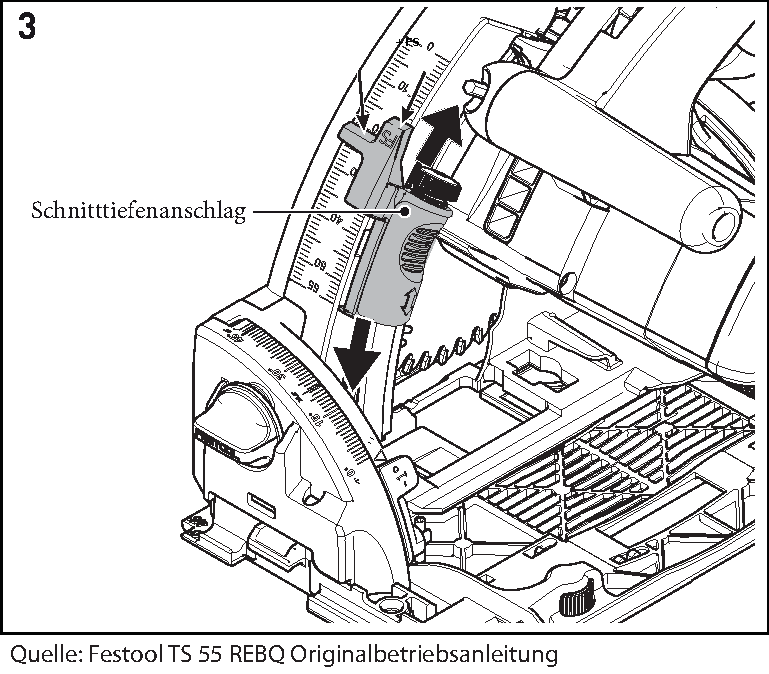
\includegraphics[width=1\textwidth]{img/festool-schnitttiefenanschlag.pdf}
	\captionof{figure}{Schnitttiefenanschlag bei Tauchsäge Festool TS 55 REBQ}
	\label{fig:schnitttiefenanschlag}
\end{minipage}


\subsection{Schnittwinkel einstellen}
\begin{minipage}{70mm}
\begin{leftbar}{Aus Festool TS 55 REBQ Handbuch, Abschnitt 7.3 (Anmerkungen in Abschnitt~\ref{quellen} beachten)}
\textbf{Schwenken zwischen 0\textdegree und 45\textdegree}
\begin{itemize}
\item[1] Schieben Sie bei Winkelschnitten das
Sichtfenster/Splitterschutz in die oberste
Position!
\item[2] Öffnen Sie die Drehknöpfe [4-1].
\item[3] Schwenken Sie das Sägeaggregat bis zum
gewünschten Schnittwinkel [4-2].
\item[4] Schließen Sie die Drehknöpfe [4-1].
\end{itemize}
\textbf{Schwenken zwischen -1\textdegree und 47\textdegree}
\begin{itemize}
\item[1] Schwenken Sie das Sägeaggregat wie oben
beschrieben in die Endlage (0\textdegree\ /45\textdegree).
\item[2] Ziehen Sie die Entriegelung [4-3] leicht heraus.
\item[3] Ziehen Sie für den -1\textdegree\ -Hinterschnitt zusätzlich die Entriegelung [4-4] heraus. Das Sägeaggregat fällt in die -1\textdegree\ /47\textdegree -Stellung.
\item[4] Schließen Sie die Drehknöpfe [4-1].
\end{itemize}
\end{leftbar}
%\vspace{30mm}
\end{minipage}
\hspace{7mm}
\begin{minipage}{90mm}
    \centering
	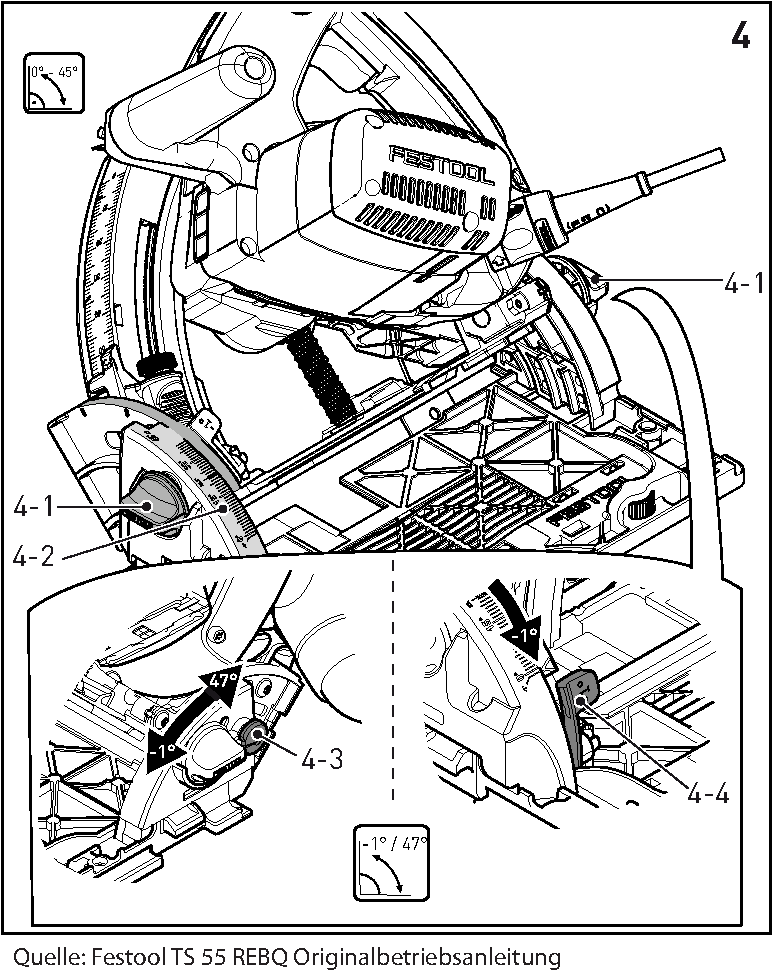
\includegraphics[width=1\textwidth]{img/festool-schnittwinkel.pdf}
	\captionof{figure}{Schnittwinkeleinstellung bei Tauchsäge Festool TS 55 REBQ}
	\label{fig:schnittwinkel}
\end{minipage}

\subsection{Sägeblatt wechseln}
\begin{minipage}{70mm}
   \begin{leftbar}{Aus Festool TS 55 REBQ Handbuch, Abschnitt 7.4 (Anmerkungen in Abschnitt~\ref{quellen} beachten)}
\textbf{Verletzungsgefahr durch heißes und scharfes Werkzeug}
Keine stumpfen und defekten Einsatzwerkzeuge verwenden. Schutzhandschuhe tragen.

\begin{itemize}
\item[1] Schwenken Sie die Maschine vor dem Sägeblattwechsel auf 0\textdegree -Stellung und stellen Sie
die maximale Schnitttiefe ein.
\item[2] Legen Sie den Hebel [5-2] bis zum Anschlag um.
\item[3] Schieben Sie die Einschaltsperre [5-1] nach
oben und drücken Sie das Sägeaggregat bis
zum Einrasten nach unten.
\item[4] Öffnen Sie die Schraube [5-5] mit dem Innensechskantschlüssel [5-3].
\item[5] Entnehmen Sie das Sägeblatt [5-7].
\item[6] Setzen Sie ein neues Sägeblatt ein.
Die Drehrichtung vom Sägeblatt [5-8]
und Maschine [5-6] müssen übereinstimmen!
\item[7] Setzen Sie den äußeren Flansch [5-9] so
ein, dass die Mitnahmezapfen in die Aussparung des inneren Flansches eingreift.
\item[8] Ziehen Sie die Schraube [5-5] fest an.
\item[9] Legen Sie den Hebel [5-2] zurück.
\end{itemize}
\end{leftbar}
%\vspace{30mm}
\end{minipage}
\hspace{7mm}
\begin{minipage}{90mm}
    \centering
	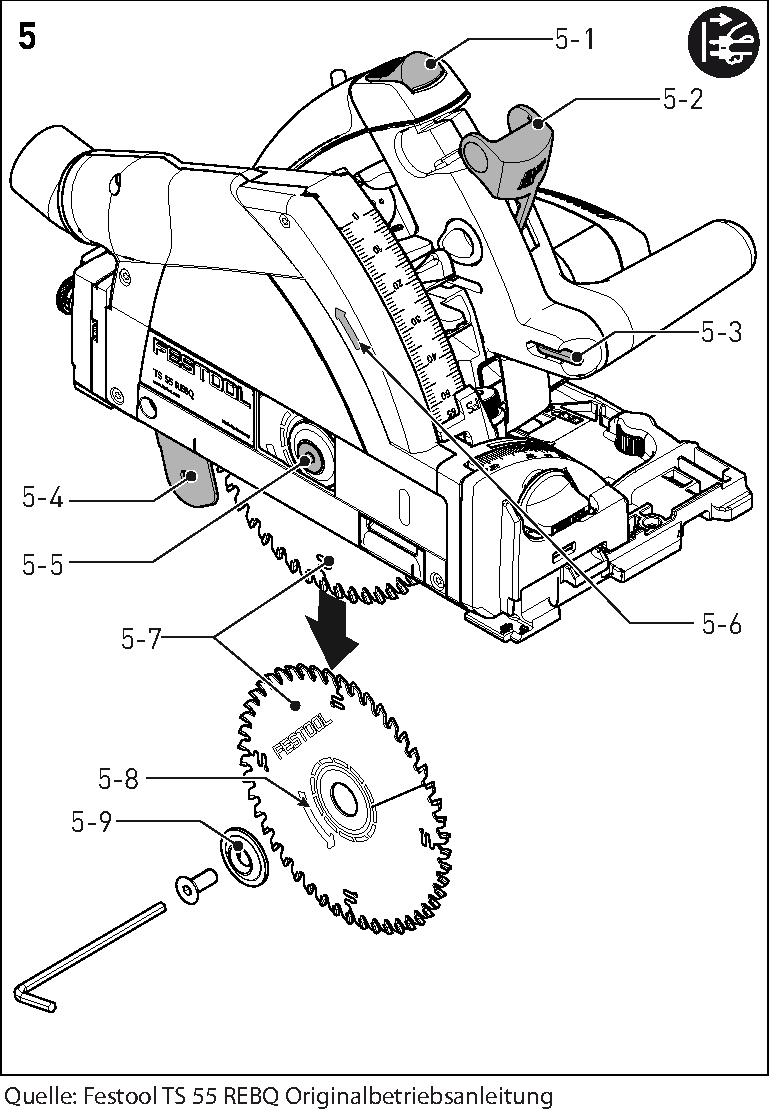
\includegraphics[width=1\textwidth]{img/festool-blattwechsel.pdf}
	\captionof{figure}{Sägeblattwechsel bei Tauchsäge Festool TS 55 REBQ}
	\label{fig:blattwechsel}
\end{minipage}


\newpage
\section{Überblickzeichnungen}
\begin{figure}[h]
	\centering
	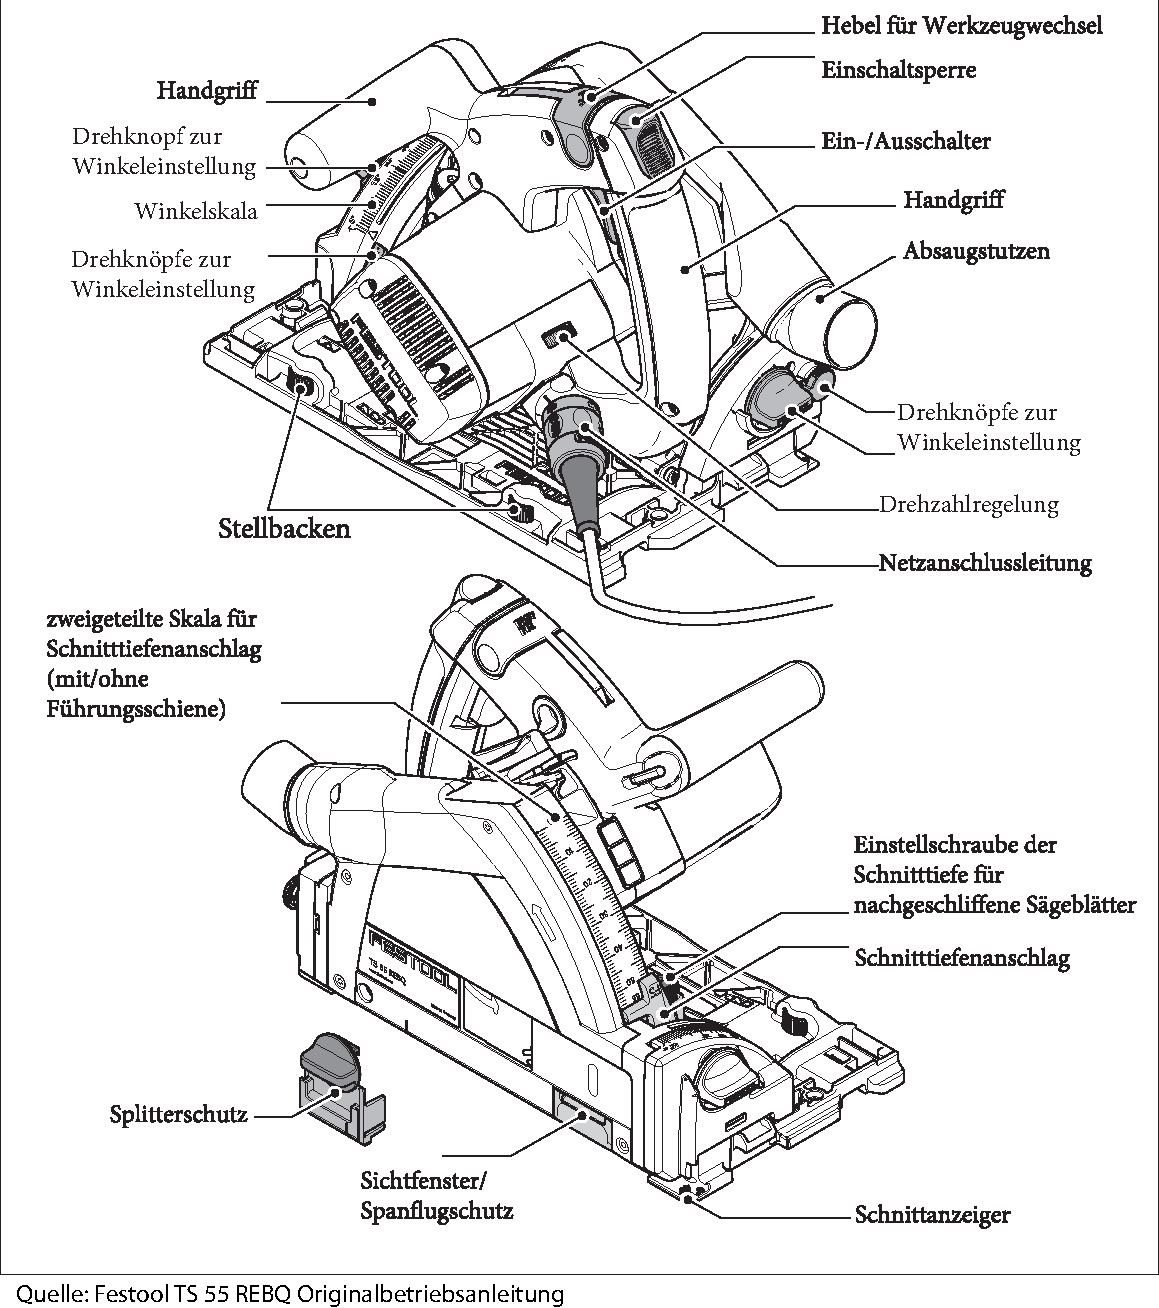
\includegraphics[width=0.9\textwidth]{img/festool-uebersicht.pdf}
	\caption{Übersicht der Tauchsäge Festool TS 55 REBQ}
	\label{fig:uebersicht}
\end{figure}












\newpage
\section{Quellen und Rechte}
\label{quellen}
Alle Rechte an Grafiken, Tabellen und Textabschnitte, welche aus der Festool Originalbetriebsanleitung übernommen wurden liegen bei Festool. Die \glqq Originalbetriebsanleitung\grqq liegt der Maschine bei und ist online auf \url{www.festool.com} zu finden. Festool hat dieses Dokument weder gelesen, noch auf Vollständigkeit oder Richtigkeit geprüft und übernimmt keine Haftung.

\end{document}
